\documentclass{suturo}

\begin{document}
    \maketitle{Vision}{13.05.2017}{}{1}{}{}{}{}

\makeatletter
\newcommand{\chapterauthor}[1]{%
  {\parindent0pt\vspace*{-47pt}%
  \linespread{2.2}\large\begin{flushright}von: #1\end{flushright}%
  \par\nobreak\vspace*{0pt}}
  \@afterheading%
}
\makeatother

\section*{Architektur und Funktion}
\chapterauthor{Tammo Wübbena}
Das Vision-Paket \footnote{im weiteren Verlauf auch Vision-Package, vision-node oder einfach Paket oder vision genannt} dient zur Akquirierung und Verarbeitung visueller Informationen durch die Kinect-Kamera des PR2-Roboters.

\begin{figure}[!htb]
        \center{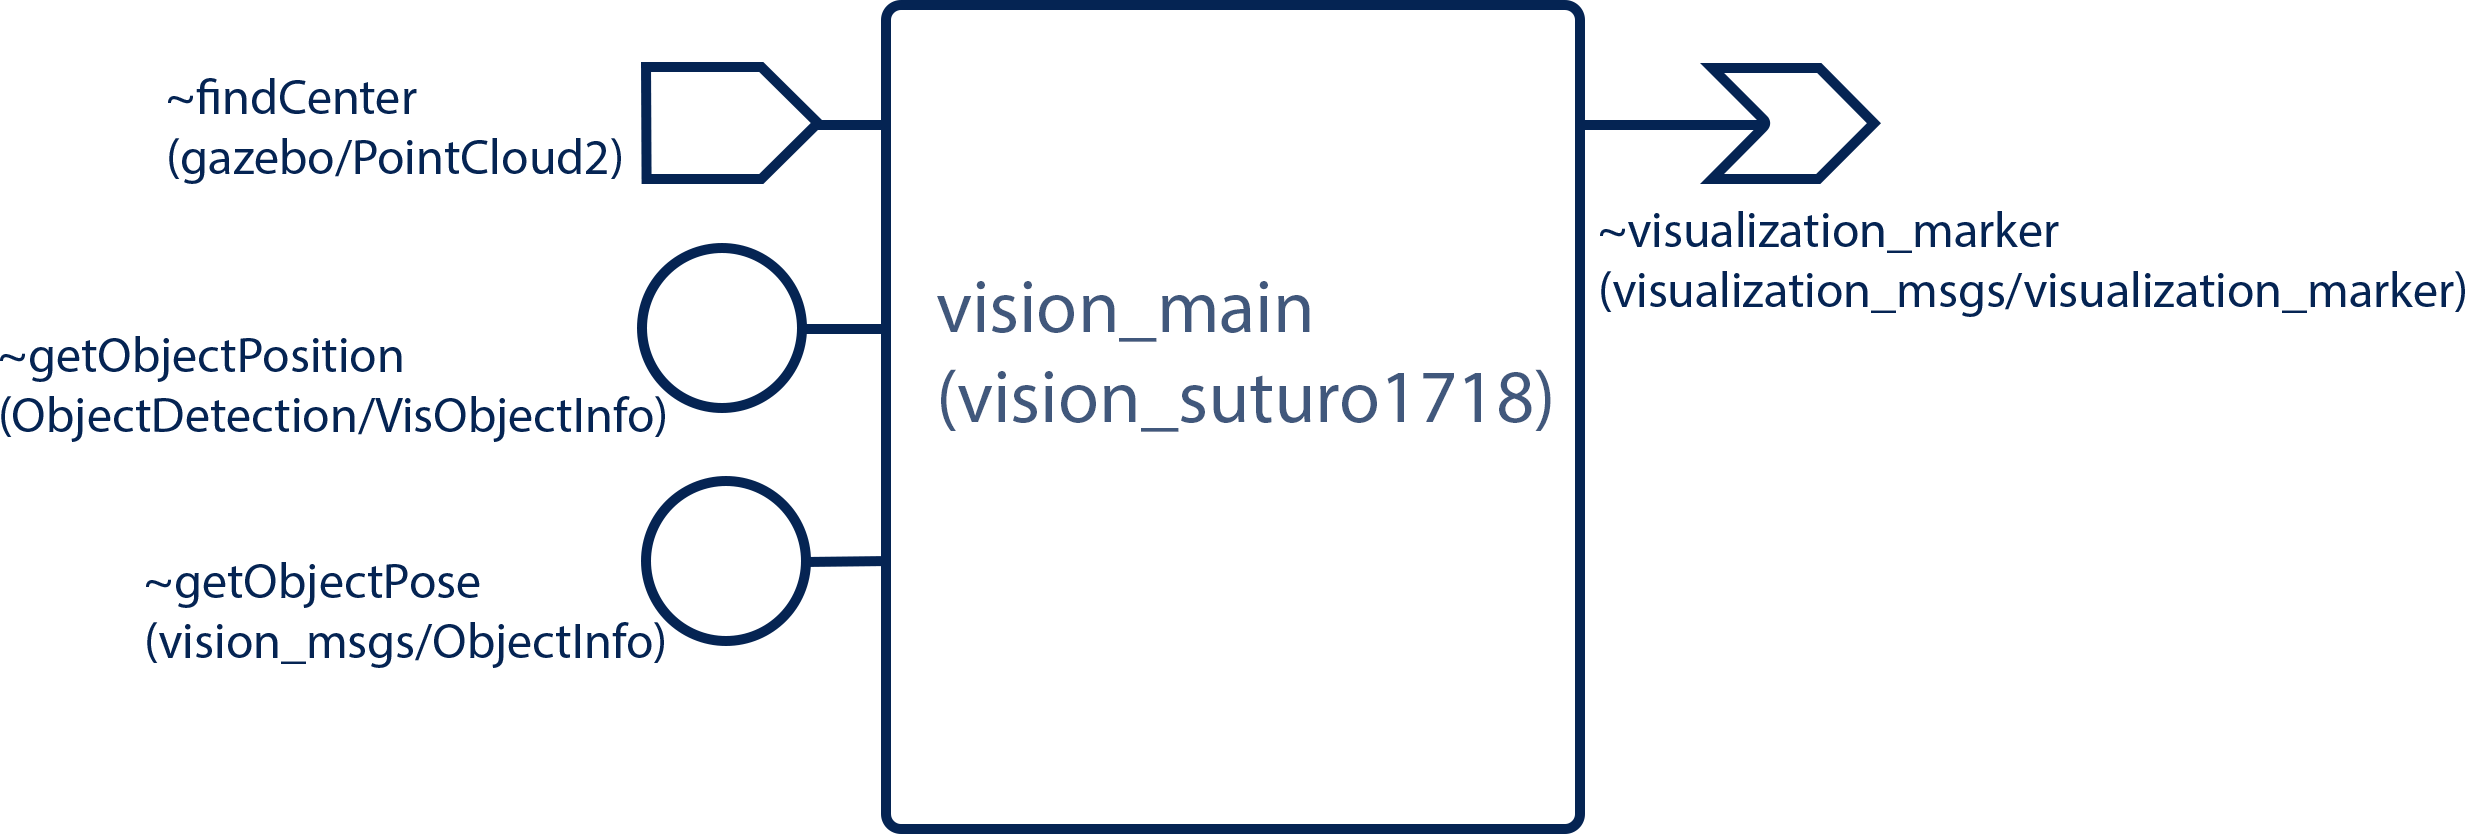
\includegraphics[width=\textwidth]
        {figures/vision_suturo_node_diagram_demo2.png}
        \caption{\label{fig:vision_node} Architektur der vision-node}}
\end{figure}
      
\section*{API}
\chapterauthor{Tammo Wübbena}

\subsection{Abkürzungen}
Für bessere Lesbarkeit haben wir typedef Kürzel verwendet:
\begin{verbatim}
typedef pcl::PointCloud<pcl::PointXYZ>::Ptr PointCloudXYZPtr;
typedef pcl::PointCloud<pcl::Normal>::Ptr PointCloudNormalPtr;
typedef pcl::PointCloud<pcl::PointXYZ> PointCloudXYZ;
typedef pcl::PointCloud<pcl::Normal> PointCloudNormal;
typedef pcl::PointIndices::Ptr PointIndices;
\end{verbatim}

\subsection{Perception}

\begin{verbatim}
#include <perception.h>
\end{verbatim}


\subsubsection{findCluster}
\begin{verbatim}
findCluster(const PointCloudXYZPtr kinect)
@params: kinect Die Punktwolke der Kinect

Description: Filtert und extrahiert einen Cluster (das gesuchte Objekt).
\end{verbatim}\label{func:findcluster}

\subsubsection{findCenterGazebo}
\begin{verbatim}
geometry_msgs::PointStamped findCenterGazebo()
@return: Künstlicher 3D-Mittelpunkt

Description: Gibt einen künstlichen Punkt zurück (Den Mittelpunkt des Modells, 
das an Gazebo übergeben wurde).
\end{verbatim}\label{func:findcentergazebo}


\subsubsection{findCenter}
\begin{verbatim}
geometry_msgs::PointStamped findCenter(const PointCloudXYZPtr object_cloud)
@param: object_cloud Eine Punktwolke (der zuvor extrahierte Cluster)
@return: 3D-Mittelpunkt der übergebenen Punktwolke

Description: Errechnet den 3D-Mittelpunkt der übergebenen Punktwolke.
\end{verbatim}\label{func:findcenter}

\subsubsection{estimateSurfaceNormals}
\begin{verbatim}
PointCloudNormalPtr estimateSurfaceNormals(PointCloudXYZPtr input)
@param: input Punktwolke, zu der die Normalen berechnet werden sollen
@return: Normalen der übergebenen Punktwolke

Description: Schätzt die Normalen einer Punktwolke ab.
\end{verbatim}\label{func:estimatesurfacenormals}

\subsubsection{createPointNormals}
\begin{verbatim}
PointCloudNormalPtr
createPointNormals(PointCloudXYZPtr input, PointCloudNormalPtr normals)
@param: input, normals Punktwolke mit zugehörigen Normalen
@return Punktwolke des Punkt-Typs pcl::PointNormal

Description: Erstellt aus einer Punktwolke (pcl::PointXYZ) und den zugörigen
Normalen (pcl::Normal) eine Punktwolke mit Punkt-Typ pcl::PointNormal.
\end{verbatim}\label{func:createpointnormals}

\subsubsection{rotatePointCloud}
\begin{verbatim}
PointCloudXYZPtr rotatePointCloud(PointCloudXYZPtr cloud) 
@param: cloud Die zu rotierende Punktwolke
@return Rotierte Punktwolke

Description: Rotiert die übergebene Punktwolke.
\end{verbatim}\label{func:rotatepointcloud}


\subsubsection{apply3DFilter}
\begin{verbatim}
PointCloudXYZPtr apply3DFilter(PointCloudXYZPtr input, float x, float y, float z)
@param: input Punktwolke, die gefiltert werden soll
		x,y,z Bereiche der Achsen für den Filter
@return Rotierte Punktwolke

Description: Filtert eine Punktwolke, indem sie nur die Punkte in einem bestimmten
Bereich ((-x,x), (-y,y), (0.0,z)) erhält.
\end{verbatim}\label{func:apply3dfilter}


\subsubsection{isStanding}
\begin{verbatim}
Nicht benutzt (legacy)

Description: Berechnet, ob ein Objekt steht oder liegt.
\end{verbatim}\label{func:isstanding}

\subsubsection{estimatePlaneIndices}
\begin{verbatim}
PointIndices estimatePlaneIndices(PointCloudXYZPtr input)
@param: input Punktwolke, deren Planare ermittelt und deren Indices gespeichert
werden sollen
@return Indices des Planar, das in der Punktwolke enthalten ist (wenn eins enthalten ist).

Description: Errechnet die Indices eines Planars einer Punktwolke.
\end{verbatim}\label{func:estimateplaneindices}

\subsubsection{extractCluster}
\begin{verbatim}
PointCloudXYZPtr extractCluster(PointCloudXYZPtr input, PointIndices indices, 
bool negative);
@param: input Punktwolke, aus der ein Cluster extrahiert werden soll
		indices Indizes der Punkte in input, die extrahiert werden sollen
		negative Setzt die flag, ob indices extrahiert werden soll (false) oder
		alle Punkte, außer den in indices angegebenen (true).
@return Objekt-Cluster aus input

Description: Extrahiert Objekt-Cluster anhand übergebener Punktwolke und
übergebenen Indices.
\end{verbatim}\label{func:extractcluster}

\subsubsection{prismSegmentation}
\begin{verbatim}
PointIndices prismSegmentation(PointCloudXYZPtr input_cloud, PointCloudXYZPtr plane)
@param: input_cloud Punktwolke, auf der Prisma-Segmentation ausgeführt werden soll
		plane Planar zur Bestimmung des Prismas zur Segmentation
@return Indizes von Objekten

Description: Errechnet Indizes zur Extraktion eines Clusters von Objekten via
Prisma-Segmentation.
\end{verbatim}\label{func:prismsegmentation}

\subsubsection{createCovarianceMatrix}
\begin{verbatim}
void createCovarianceMatrix(PointCloudXYZ input, Eigen::Matrix3f covariance_matrix);
@param: input Punktwolke, für die eine Kovarianz-Matrix erstellt wird
		covariance_matrix Die zu errechnende Kovarianz-Matrix
@return Kovarianz-Matrix einer Punktwolke.

Description: Errechnet Kovarianz-Matrix einer Punktwolke.
\end{verbatim}\label{func:createcovariancematrix}

\subsubsection{mlsFilter}
\begin{verbatim}
PointCloudXYZPtr mlsFilter(PointCloudXYZPtr input);
@param: input Punktwolke, die mittels Moving-Least-Squares-Algorithmus geglättet wird
@return Geglättete Punktwolke

Description: Glättet Punktwolke mit MLS-Algorithmus.
\end{verbatim}\label{func:mlsfilter}

\subsubsection{voxelGridFilter}
\begin{verbatim}
PointCloudXYZPtr voxelGridFilter(PointCloudXYZPtr input)
@param: input Zu filternde Punktwolke
@return Mit einem Voxel-Gitter gefilterterte (und damit gedownsamplete) Punktwolke

Description: Filtert eine Punktwolke mit dem Voxel-Gitter-Filter.
\end{verbatim}\label{func:voxelgridfilter}

\subsubsection{outlierRemoval}
\begin{verbatim}
PointCloudXYZPtr outlierRemoval(PointCloudXYZPtr input)
@param: input Punktwolke, die von Rauschen befreit werden soll
@return Gefilterte Punktwolke

Description: Entfernt Punkte aus Punktwolke, die als zu weit außen liegend
(outlier) oder als Rauschen erkannt werden.
\end{verbatim}\label{func:outlierremoval}

\subsubsection{checkModelPresence}
\begin{verbatim}
int checkModelPresence(PointCloudXYZPtr scene);
@param: scene Punktwolke, in der ein Objekt gefunden werden soll
@return 0 Wenn Objekt gefunden, 1 wenn nicht

Description: Überprüft, ob ein gewisses Model in einer Punktwolke (Szene) existiert.
\end{verbatim}\label{func:checkmodelpresence}

\subsubsection{initialAlignmentAndICP}
\begin{verbatim}
int initialAlignmentAndICP();
@return: 0 wenn Objekt in einer Szene liegt, 1 sonst
Description: Errechnet mit Initial Alignment und dem
Iterative-Closest-Point-Algorithmus, ob ein Objekt in einer Szene steht oder liegt.
\end{verbatim}\label{func:initialalignmentandicp}


\subsection{saving}
Hilfsfunktionen zum Speichern von Punktwolken als .PCD-Dateien.

\begin{verbatim}
void savePointCloudXYZ(pcl::PointCloud<pcl::PointXYZ>::Ptr cloud);
void savePointCloudXYZNamed(pcl::PointCloud<pcl::PointXYZ>::Ptr cloud, char *filename);
void savePointCloudNormal(pcl::PointCloud<pcl::Normal>::Ptr cloud);
void savePointCloudPointNormal(pcl::PointCloud<pcl::PointNormal>::Ptr cloud);
void savePointCloud(pcl::PointCloud<pcl::PointXYZ>::Ptr objects,
                    pcl::PointCloud<pcl::PointXYZ>::Ptr kinect,
                    pcl::PointCloud<pcl::Normal>::Ptr normals);
\end{verbatim}

\subsection{viewer}
Hilfsfunktionen zur Darstellung von Punktwolken.

\begin{verbatim}
void visualizePointCloud(pcl::PointCloud<pcl::PointXYZ> cloud);
void visualizeNormals(pcl::PointCloud<pcl::PointXYZ>::Ptr cloud, 			 	
									pcl::PointCloud<pcl::Normal>::ConstPtr normals);
\end{verbatim}

\subsection{conversion}
Hilfsfunktionen zur Konvertierung von Punktwolken (Matrizen, andere Punktwolken-Formate, ...).

\begin{verbatim}
cv::Mat PointCloud2cvMat(pycl::PointCloud<pcl::PointXYZ>::Ptr input)
\end{verbatim}
\subsection{globals}
Globale Variablen und Konstanten für den leichteren Zugriff.

\begin{verbatim}
const char* SIM_KINECT_POINTS_FRAME = "/head_mount_kinect/depth_registered/points";
const char* REAL_KINECT_POINTS_FRAME = "/kinect_head/depth_registered/points";

const char* GREEN_MSG_COL = "\x1B[32m";


gazebo_msgs::GetModelState getmodelstate;
ros::ServiceClient client;
std::string
        error_message; // Wird durch den Object Position Service mit ausgegeben

pcl::PointCloud<pcl::PointXYZ>::Ptr kinect_global(new pcl::PointCloud<pcl::PointXYZ>);
pcl::PointCloud<pcl::PointXYZ>::Ptr objects_global(new pcl::PointCloud<pcl::PointXYZ>);
pcl::PointCloud<pcl::Normal>::Ptr normals_global(new pcl::PointCloud<pcl::Normal>);
pcl::PointCloud<pcl::PointNormal>::Ptr pointnormals_global(new
												pcl::PointCloud<pcl::PointNormal>);
pcl::PointCloud<pcl::PointXYZ>::Ptr mesh_global(new pcl::PointCloud<pcl::PointXYZ>);
pcl::PointCloud<pcl::PointXYZ>::Ptr objects_rotated_global(new 	
											 	pcl::PointCloud<pcl::PointXYZ>);

geometry_msgs::PointStamped centroid_stamped;
\end{verbatim}


\section*{Schnittstellen}
\chapterauthor{Alexander Link}

\subsection*{Service Server vision\_main/objectPoint}
\begin{verbatim}
VisObjectInfo.srv
@request: -
@response: ObjectDetection msg (string error, geometry_msgs/PointStamped position)
\end{verbatim}
Gibt die Position des Eistees aus. Kann bei Problemen unterschiedliche Fehlermeldungen zurückgeben.
\\ \\
Wird in einem Durchgang zwei mal von Planning aufgerufen. Ein mal zur grundsätzlichen Feststellung der Position des Objekts, ein zweites mal zur Überprüfung, ob sich die Position des Objekts geändert hat.

\subsection*{Service Server vision\_main/objectPose}
\begin{verbatim}
GetObjectInfo.srv
@request: -
@response: ObjectInformation msg (int32 isStanding, string information)
\end{verbatim}
Sollte ursprünglich ausgeben, ob der Eistee steht, oder liegt. Soll stattdessen aktuell ausgeben, ob der Eistee im Sichtfeld ist, oder nicht.
\\ \\
Wird aktuell nicht verwendet.

\subsection*{Subscriber REAL\_KINECT\_POINTS\_FRAME}
\begin{verbatim}
@response: PointCloudXYZPtr kinect
\end{verbatim}
Gibt eine Punktwolke unseres Sichtfelds zurück.
\\ \\
Wird stetig immer wieder benutzt, um eine möglichst aktuelle Position des Objekts beizubehalten.

\subsection*{Service Client gazebo/get\_model\_state}
\begin{verbatim}
gazebo_msgs/GetModelState.srv
@request: -
@response:  string model_name,
            string relative_entity_name,
            std_msgs/Header header (uint32 seq, time stamp, string frame_id),
            geometry_msgs/Pose pose (...),
            geometry_msgs/Twist twist (...),
            bool success,
            string status_message
\end{verbatim}
Gibt Informationen über das gesuchte Objekt direkt aus gazebo aus.
\\ \\
Wird benutzt, um bei Problemen in der Simulation anstelle der vom kinect erkannten Daten auf die direkten Daten aus gazebo ausweichen zu können, an denen der Kinect-Sensor unbeteiligt ist.

\section*{Programmablauf}

Ein Subscriber empfängt die zu verarbeitenden Punktwolken des Kinect-Sensors und führt jedes mal die Funktion findCluster in perception.h aus. Diese führt dann unter Verwendung der eingegangenen Daten unsere Filter und Segementierungsprozesse in einer festen Reihenfolge aus:
\linebreak
\begin{itemize} 
\item Ein Stichpunkt 
\item Noch ein Stichpunkt 
\end{itemize}

\end{document}
